\chapter{Results}%
\label{chap:Results}

In this chapter, the results gathered from our evaluation of the dynamic window against 
the tumbling window will be discussed by the order of the workloads. The workload 
evaluations are run multiple times for consistency of results. We will first 
discuss the workload for latency measurement, followed by periodic workload and 
finally the completeness measurement. For each workload results, we elaborate 
and discuss in details the shortcomings of the evaluation methods and the 
possible outlier situations for which the evaluation result would not agree with.



\section{Workload for latency measurement}%



\label{sec:Workload for latency measurement}
\begin{figure*}
    \begin{subfigure}[b]{0.5\textwidth}
        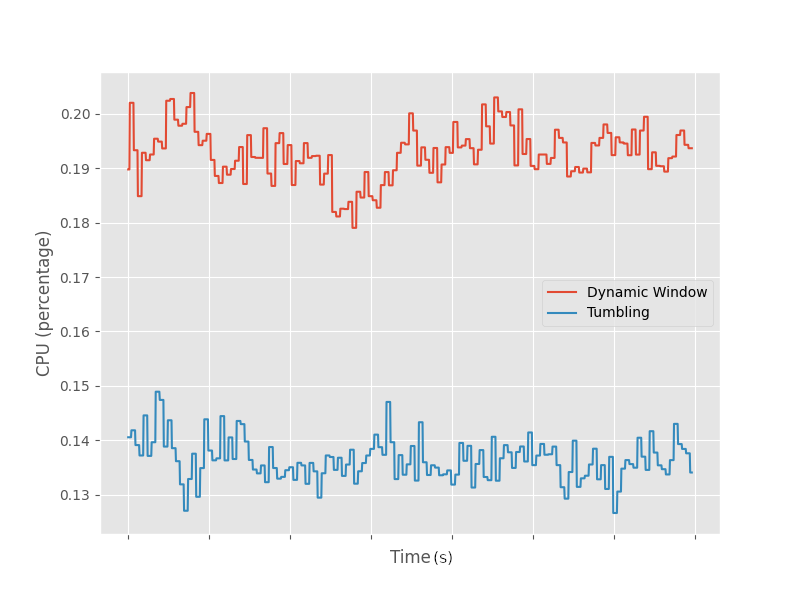
\includegraphics[width=\textwidth]{fig/constant-rate/cpu_comparison.png}
        \caption{}
        \label{fig:constant_cpu}
    \end{subfigure}
    \hfill 
    \begin{subfigure}[b]{0.5\textwidth}
        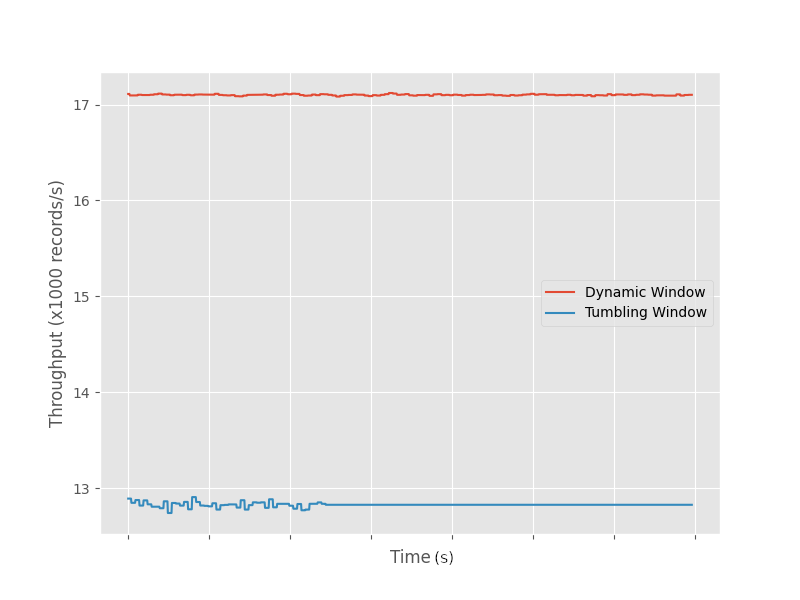
\includegraphics[width=\textwidth]{fig/constant-rate/throughput_comparison.png}
        \caption{}
        \label{fig:constant_thorughput}
    \end{subfigure}
    %%
    \begin{subfigure}[b]{0.5\textwidth}
        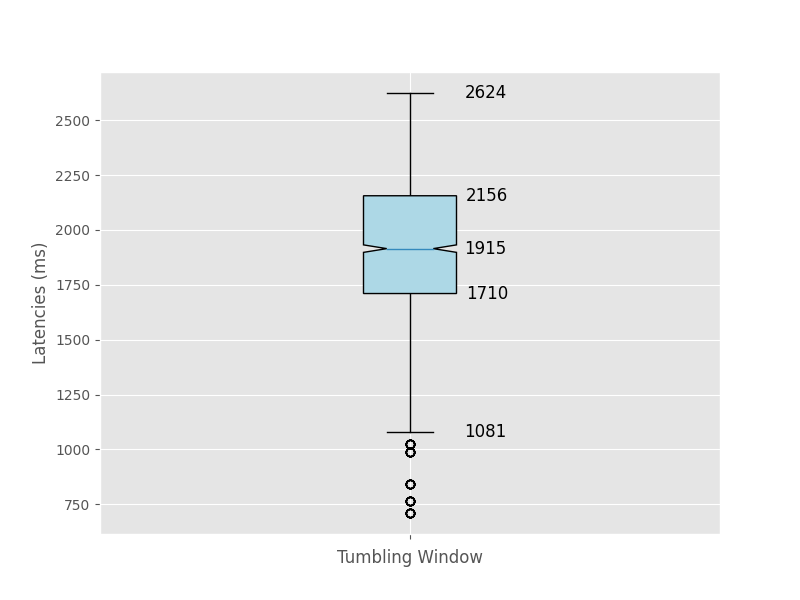
\includegraphics[width=\textwidth]{fig/constant-rate/TumblingWindow_latency_boxplot.png}
        \caption{}
        \label{fig:constant_tumb_boxplot}
    \end{subfigure}
    \hfill 
    \begin{subfigure}[b]{0.5\textwidth}
        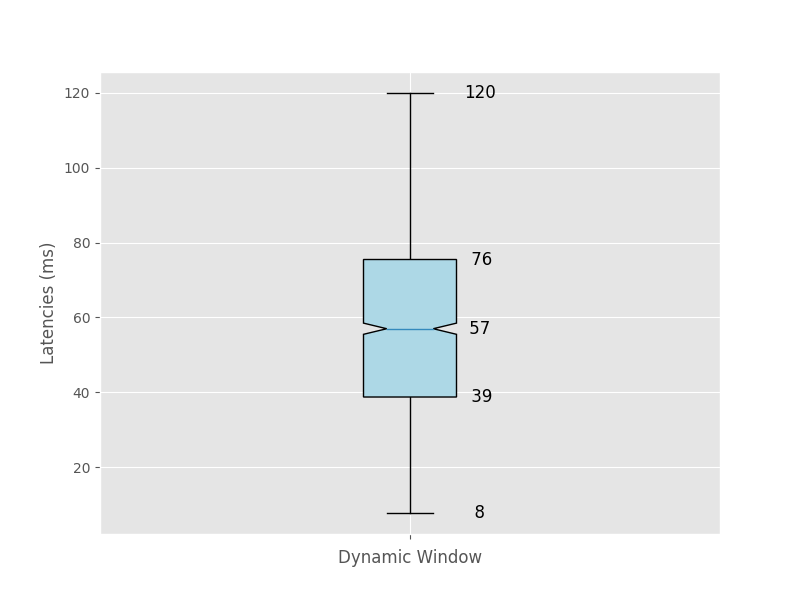
\includegraphics[width=\textwidth]{fig/constant-rate/DynamicWindow_latency_boxplot.png}
        \caption{}
        \label{fig:constant_dynamic_boxplot}
    \end{subfigure}
    \caption{Metrics measurements for latency workload.}%
    \label{fig:cpucomparison}
\end{figure*}



